\documentclass[12pt]{article}
\usepackage{color}
\usepackage{graphicx}
\usepackage{booktabs}
\usepackage{amsmath}
\usepackage[utf8]{inputenc}
%\usepackage[german]{babel}
\usepackage{multirow}
\usepackage{siunitx}
\usepackage{pbox}
%\usepackage{tabularx}
\usepackage{multirow}
\usepackage{float}
\usepackage{amssymb,amsmath}
\makeatletter
\def\maketag@@@#1{\hbox{\m@th\normalfont\normalsize#1}}
\makeatother
\setlength{\parindent}{0pt}

%\addtolength{\textwidth}{1in}
%\addtolength{\textheight}{1in}
%\addtolength{\evensidemargin}{0.5in}
%\addtolength{\oddsidemargin}{-0.5in}
%\addtolength{\topmargin}{-0.6in}
%\addtolength{\bottommargin}{0.4in}


\usepackage[top = 2.50cm, bottom = 2.50cm, left = 2.75cm, right = 2.50cm]{geometry}

\renewcommand{\floatpagefraction}{1.0}


\begin{document}
\title{PHY118/119 \\ {\bf Starre Körper}}
\author{Assistent: Simon Flury \\E-mail: simon.flury@uzh.ch\\ }
\maketitle

\section{Wichtig!!!}
Dieses Dokument ist kein offizielles Dokument, es ist weder von Prof.Kilminster noch vom Hauptassistenten abgesegnet, somit kann sich nicht darauf bezogen werden und es wird auch keine Haftung für Fehler übernommen. Es dient einzig und allein als Lernunterstützung von mir an euch und bezieht sich ausschliesslich auf meine Übungsstunde.

\section{Rotation/Translation starrer Körper}
Ein starrer Körper im Sinne der klassischen Mechanik, beschreibt ein Modell eines nicht verformbaren Körpers. Diese Nichtverformbarkeit ist eine Idealisierung, in der Realität verformt sich jedes Objekt ein wenig, jedoch meist nur so wenig, dass wir die Verformung vernachlässigen können und die Behandlung als starren Körper gute Näherungen liefert. Der Körper an sich muss nicht zwingend eine kontinuierliche Massenverteilung aufweisen, sondern kann auch ein System von diskreten Massenpunkten sein.\\
\\
\textbf{Definition (starrer Körper):}\\
Bei einem starren Körper bleiben die Abstände zwischen den einzelnen Molekülen konstant:
\begin{equation}
d = |\vec{r_i} - \vec{r_j}| = \mathrm{const}
\end{equation}
Aufteilung der Bewegung in Translation und Rotation\\
\clearpage

\textbf{nur Rotation}\\
\begin{figure}[H]
  \centering{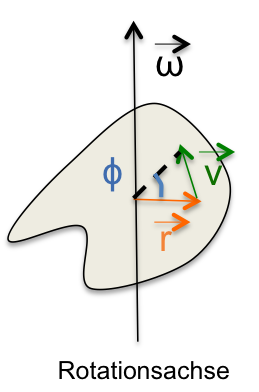
\includegraphics[width=0.2\textwidth]{Grafik1.png}}
  \caption{Schema Rotationsbewegung.}
  \label{fig:1teil}
\end{figure} 
reine Rotationsbewegung um feste Rotationsachse. Betrachte zeitabhängigen Winkel $\varphi (t)$. Die Winkelgeschwindigkeit bzw. Kreisfrequenz ist gegeben durch $\omega = \dfrac{d \varphi}{dt} = \dfrac{2\pi}{T}$. Da wir im Modell des starren Körpers die Abstände als fix betrachten gilt: \textbf{Winkelgeschwindigkeit ist überall gleich.}\\
Vektoriell betrachtet folgt:
\begin{equation}
\vec{v} = \vec{\omega} \times \vec{R}
\end{equation}
(bitte seit euch bewusst was dies bedeutet, nämlich das $\vec{v}$ senkrecht auf $\vec{\omega}$ und $\vec{R}$ steht, sprich normal zur von Omega und R aufgespannten Ebene.)\\
\\
zudem gilt:
\begin{itemize}
\item bei einer Rotation zeigt $\vec{\omega}$ immer in die gleiche Richtung.
\item Im allgemeinen kann $\vec{\omega}$ seine Richtng ändern.
\end{itemize}

\begin{figure}[H]
  \centering{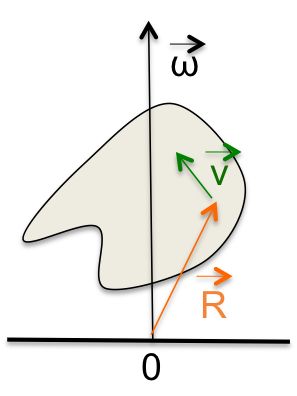
\includegraphics[width=0.2\textwidth]{Grafik2.png}}
  \caption{Vektorschema.}
  \label{fig:1teil}
\end{figure} 

\clearpage

\textbf{nur Translation}
\begin{figure}[H]
  \centering{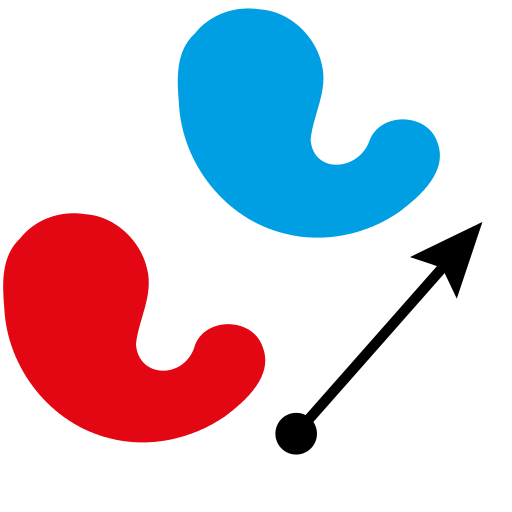
\includegraphics[width=0.2\textwidth]{Grafik2_2.png}}
  \label{fig:1teil}
\end{figure} 

Bei der reinen Translation gibt eine beliebige Geschwindigkeit in einem Punkt des Körpers die Translationsgeschwindigkeit des ganzen Körpers an da sie, wieder aufgrund der Invarianz der Abstände, als Schwerpunktsgeschwindigkeit aufgefasst werden kann: 
\begin{equation}
\vec{v_i} = \vec{v_s} \qquad \forall i \in \mathbb{N}
\end{equation}
\\
\\
\textbf{Kinetische Energie von Rotation und Translation}
\\
\\ kinetische Energie der Translation: $E_{kin}^{trans} = \sum \dfrac{1}{2}m_i v_i^2 = \left(\sum \dfrac{1}{2} m_i \right) v_s^2 = \dfrac{M}{2} v_s^2$ wobei wir verwendet haben, dass $v_i = v_s$ und $\sum m_i = M$ ist. Somit erhalten wir für die Translation:
\begin{equation}
E_{kin}^{trans} = \dfrac{M}{2} v_s^2
\end{equation}
\\
\\
kinetische Energie der Rotation: $E_{kin}^{rot} = \sum \dfrac{1}{2} m_i v_i^2 = \sum \dfrac{1}{2} m_i r_i^2 \omega^2 = \dfrac{1}{2} I \cdot \omega^2$ wobei $I$ das Trägheitsmoment bezüglich einer fixen Drehachse ist. Somit erhalten wir für die Rotation:
\begin{equation}
E_{kin}^{rot} = \dfrac{1}{2} I \cdot \omega^2
\end{equation}
vorsicht $r_i$ bezeichnet immer den Abstand senkrecht zur Drehachse $r_i = R sin(\theta)$, zur Veranschaulichung betrachtet folgendes Schema:

\begin{figure}[H]
  \centering{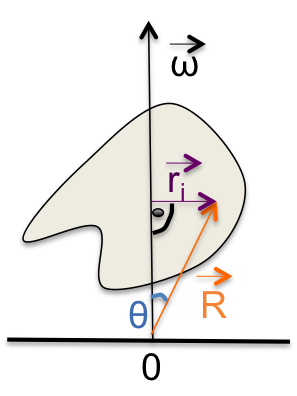
\includegraphics[width=0.2\textwidth]{Grafik3.png}}
  \label{fig:1teil}
\end{figure}
somit gilt $|\vec{v}| = |\vec{\omega} \times \vec{R}| = \omega \cdot R \cdot sin(\theta) = \omega \cdot r_i$

\section{Massenträgheitsmoment}

Das Massenträgheitsmoment ist das Äquivalent der Rotation zur Trägenmasse der Translation und wird immer bezüglich einer fixen Drehachse angegeben $I_k = \sum m_i r_i^2$ bezüglich der $k$-Achse.
(Die Trägheitsmomente verschiedener starre Körper bezüglich verschiedener Drehachsen sind tabelliert und es wird nicht von euch verlangt, dass ihr sie berechnen könnt. Trotzdem zeige ich euch unten an einem einfachen Beispiel wie das geht.)

\textbf{Wichtige Massenträgheitsmomente}
\begin{itemize}
\item Punktmasse im Abstand $r$ um Drehachse: $I = m\cdot r^2$
\item Vollzylinder um Symmetrieachse: $I = \dfrac{1}{2}m\cdot r^2$
\item Hohlzylinder um Symmetrieachse: $I = m \dfrac{r_1^2 + r_2^2}{2}$
\item dünner Stab um Querachse: $I = \dfrac{1}{12}m \cdot l^2$
\item Vollkugel: $I = \dfrac{2}{5}m \cdot r^2$
\item Kugelschale: $I = \dfrac{2}{3}m \cdot r^2$
\end{itemize}

\subsection{Beispiel: Trägheitsmoment von rotierendem Stab}

\begin{figure}[H]
  \centering{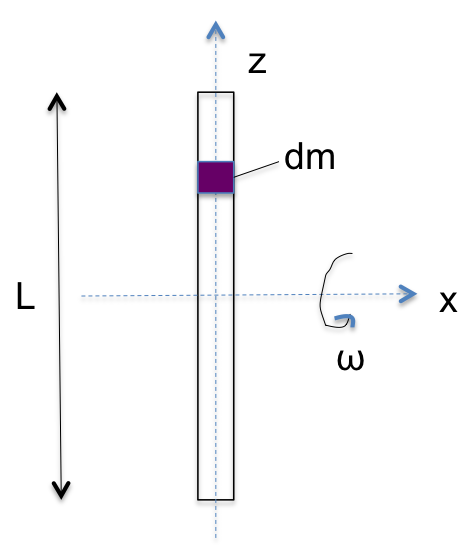
\includegraphics[width=0.2\textwidth]{Grafik4.png}}
  \caption{dünner Stab welcher um x-Achse rotiert.}
  \label{fig:1teil}
\end{figure} 

Um das Trägheitsmoment zu berechnen gehen wir von einem infinitesimalen Massenelement aus und integrieren über die gesamte Masse des Stabes. $m_i \rightarrow dm$ also $\sum m_i r_i^2 \rightarrow \int dm \cdot r^2$.\\
Folgende Zusammenhänge werden wir verwenden: $dm = \rho \cdot dV = \rho \cdot dz \cdot A$ wobei $A = \pi R^2$ die Querschnittsfläche des Stabes bezeichnet.
\begin{equation}
I_x = \int_{-L/2}^{L/2} z^2 \rho dz \pi R^2 = \left. \dfrac{z^3}{3} \right|_{-L/2}^{L/2} \cdot \rho \pi R^2 = \dfrac{L^3}{12} \cdot \rho \pi R^2
\end{equation}
verwenden wir nun noch $M = \rho V = \rho L \pi R^2$ und erhalten für das Massenträgheitsmoment bezüglich der Querachse eines dünnen Stabes:
\begin{equation}
I_x = \dfrac{1}{12} ML^2
\end{equation}
\\
\\
\textbf{Der Satz von Steiner}
\\
Meistens wollen wir Rotationen betrachten um Achsen welche nicht durch den Schwerpunkt gehen. Nun stellt sich natürlich die Frage, wie man das Trägheitsmoment für solche Rotationen berechnet.\\
$I_s$ bezeichnet hierbei das Trägheitsmoment bei Rotation um den Schwerpunkt und $I$ um eine beliebige Achse. Der Satz von Steiner besagt nun:
\begin{equation}
I = I_s + M \cdot s^2
\end{equation}
weobei $s$ die Distanz zwischen $I$ und $I_s$ bezeichnet und $M$ die Gesamtmasse.

\section{Dynamik der Drehbewegung}
Bisher haben wir immer die Energie betrachtet, nun wollen wir uns den Kräften zuwenden. Betrachten wir dazu das 2.Newton'sche Axiom für ein System, wobei wir nur äussere Kräfte betrachten.
\begin{equation}
\dfrac{p_i}{dt} = \vec{F_i} \rightarrow \vec{v_i} \times \dfrac{d\vec{p_i}}{dt} = \vec{r_i} \times \vec{F_i}
\end{equation}
somit folgt
\begin{equation}
\dfrac{d}{dt} (\vec{r_i} \times \vec{p_i}) = \dfrac{d \vec{r_i}}{dt} \times \vec{p_i} + \vec{r_i} \times \dfrac{d \vec{p_i}}{dt} = \vec{r_i} \times \dfrac{d \vec{p_i}}{dt}
\end{equation}
Achtung $\vec{a} \times \vec{a} = 0$ und $\vec{p_i} = m \dfrac{d \vec{r_i}}{dt}$

nun werden wir einige Grössen definieren:

\begin{itemize}
\item \textbf{Drehimpuls} $\vec{L_i} = \vec{r_i} \times \vec{p_i}$
\item \textbf{Drehmoment} $\vec{M_i} = \vec{r_i} \times \vec{F_i}$
\end{itemize}
analog dazu ist der Gesamtdrehimpuls $\vec{L} = \sum_{i} (\vec{r_i} \times \vec{P_i})$ und das Gesamtdrehmoment $\vec{M} = \sum_{i} (\vec{r_i} \times \vec{F_i})$
\\
\\
daraus folgt nun direkt aus (10) der bekannte \textbf{Drallsatz};
\begin{equation}
\dfrac{d\vec{L}}{dt} = \vec{M}
\end{equation}


Der Drehimpuls ist wie der Impuls eine Erhaltungsgrösse. Dies bedeutet, dass der Gesamtdrehimpuls zu jeder Zeit gleich ist, $\vec{L}_{initial} =\vec{L}_{final}$
\\
\clearpage

\textbf{Drehimpulserhaltung}\\
Formal: wirken auf ein System von N Massepunkten mit Gesamtdrehimpuls $\vec{L} = \sum_{i} \vec{L_i}$ keine äusseren Momente $\vec{M_a} = 0$ folgt unter verwendung des Drallsatzes direkt:

\begin{equation}
\dfrac{d \vec{L}}{dt} = \vec{M_a} = 0 \quad \rightarrow \quad \vec{L} = const
\end{equation}
\\
\\
Wir wollen am Beispiel einer rotierenden Scheibe die Rollbedingung herleiten.

\begin{figure}[H]
  \centering{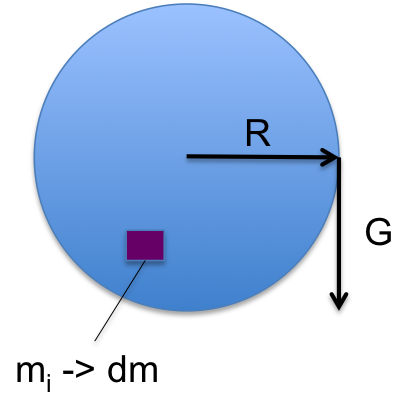
\includegraphics[width=0.15\textwidth]{Grafik5.png}}
  \label{fig:1teil}
\end{figure} 
 wobei $\vec{R}$ der Radius und $\vec{G}$ die Gewichtskraft ist. Durch diese Gewichtskraft wird auf die Scheibe ein Drehmoment ausgeübt $\vec{M} = \vec{R} \times \vec{G}$. Da die Vektoren senkrecht stehen gilt $M = R \cdot G$.\\
 Betrachten wir nun den Drehimpuls $\vec{L} = \sum_{i} \vec{r_i} \times \vec{p_i} = \sum_{i} \vec{r_i} \times m_i \vec{v_i} = \sum_{i} \vec{r_i} \times m_i r_i \omega_i$ und auch da die Vektoren senkrecht zueinander stehen $\sum_{i} m_i r_i^2 \cdot \omega = I_z \cdot \omega$ für starre Körper mit fester Drehachse $\vec{\omega}$\\
 Wenn wir nun den Drallsatz verwenden, erhalten wir: $\dfrac{d \vec{L}}{dt} = I \cdot \dfrac{d \omega}{dt} = M$
\\
\\
Stellen wir uns nun vor, auf dieser Scheibe sei ein Seil aufgewickelt an welchem unten ein Gewicht hängt. Dann wirkt die Gewichtskraft $\vec{G}$ nach unten, das Gewicht übt eine Zugkraft $\vec{F_2}$ auf das Seil aus und vom Seil geht eine Gegenkraft $\vec{F_1}$ nach unten.

\begin{figure}[H]
  \centering{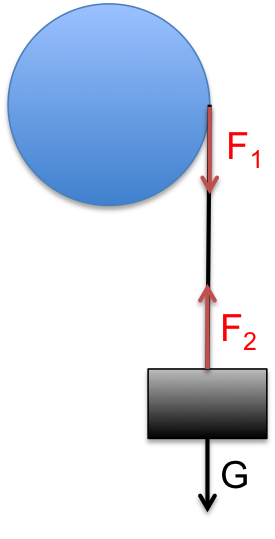
\includegraphics[width=0.15\textwidth]{Grafik6.png}}
  \label{fig:1teil}
\end{figure} 
wir haben nun also vom fallenden Körper $ F_2 - G = ma$ und von der Rotation der Scheibe $ I \cdot \dfrac{d\omega}{dt} = R \cdot F_1$. Als Zwangsbedingung gilt, dass der Faden zu jedem Zeitpunkt gestreckt ist. Daraus erhalten wir letzten Endes $F_1 = -F_2$ und somit unsere Rollbedinung:
\begin{equation}
a = R \cdot \dfrac{d\omega}{dt}
\end{equation}

\section{Rollen und Gleiten}

\begin{figure}[H]
  \centering{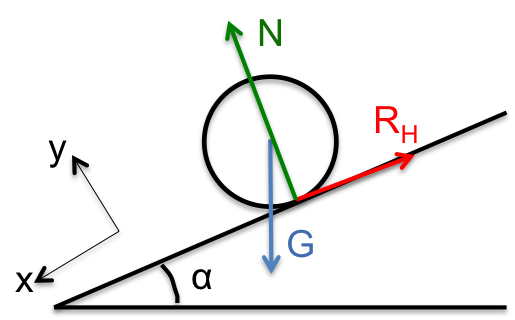
\includegraphics[width=0.4\textwidth]{Grafikrolle.png}}
  \label{fig:1teil}
\end{figure} 

Wir wollen nun ein reines Rollen auf einer schiefen Ebene betrachten.\\
Die Haftreibung ist gegeben durch: $R_H \leq \mu_H \cdot N$. Die Bewegungsgleichungen lauten nun:\\
Für die Translation in x-Richtung
\begin{equation}
m \ddot{x_s} = Gsin(\alpha) - R_H
\end{equation}
und für Rotation
\begin{equation}
M = \dfrac{dL}{dt} = I_z \dfrac{d \omega}{dt} = r \cdot R_H
\end{equation}
wenn wir nun die Rollbedinung benutzen erhalten wir:
\begin{equation}
a = \ddot{x_s} = r \dfrac{d \omega}{dt} = r^2 \dfrac{R_H}{I_z} = \dfrac{r^2}{I_z} (G sin(\alpha) - m \ddot{x_s}) = \dfrac{m r^2}{I_z} (g \cdot sin(\alpha) - \ddot{x_s})
\end{equation}
somit erhalten wir \begin{equation}
\ddot{x_s} = \dfrac{g \cdot sin(\alpha)}{1 + \dfrac{I_z}{mr^2}}
\end{equation}
Wir sehen also, wenn zwei Körper gleicher Masse und gleichem Radius unterschiedlich Rollen, müssen sie unterschiedliche Massenträgheitsmomente haben, somit spielt die Geometrie beim Rollvorgang eine wichtige Rolle.
\\
\\
Betrachten wir nun noch den Fall, wenn wir einen sich bereits in Rotation befindenden Zylinder auf eine schräge Ebene aufsetzten lassen. (ihr könnt genau die gleiche Grafik betrachten, nur das der Körper zu Beginn schon eine Rotationgeschwindigkeit hat.)\\
Es gilt: $I_z = \dfrac{1}{2} mr^2$ für Zylinder, $M = \dfrac{dL}{dt} = I_z \cdot \dfrac{d \omega}{dt} = -r \cdot R_G$ das Minus kommt daher, dass die Reibungskraft ja in negative x-Richtung zeigt. Wenn wir uns die Kräfte anschauen bekommen wir folgende Bewegungsgleichungen für die Translation in x- und y-Richtung:
\begin{equation}
m \ddot{x_s} = Gsin(\alpha) -R_G
\end{equation}
\begin{equation}
m \ddot{y_s} = -Gcos(\alpha) + N = 0
\end{equation}
\clearpage
aus den vorhergehenden Gleichungen und Überlegungen erhalten wir folgende Relationen:\\
$N = Gcos(\alpha)$\\
$R_G = \mu_G N = \mu_G G cos(\alpha)$\\
$I_z \dot{\omega} + rR_G = 0 \rightarrow \omega = \omega_0 - \dfrac{\mu_G G cos(\alpha)r}{I_z} \cdot t$ ($\omega_o$ ist einfach die Anfangswinkelgeschwindigkeit vor dem Aufsetzen)\\
Verwenden wir die Anfangsbedingungen $x_s(0) = 0$ und $v_s(0) = 0$ bekommen wir für die Geschwindigkeit in x-Richtung:
\begin{equation}
v_x = g\cdot (sin(\alpha) - \mu_G cos(\alpha)) \cdot t
\end{equation}
Daraus ergeben sich nun drei Fälle:\\
\\
\textbf{Fall 1}: $\mu_G > tan(\alpha) \rightarrow$ Zylinder bewegt sich nach oben.\\
\textbf{Fall 2}: $\mu_G < tan(\alpha) \rightarrow$ Zylinder bewegt sich nach unten.\\
\textbf{Fall 3}: $\mu_G = tan(\alpha) \rightarrow$ Zylinder rotiert an Ort und Stelle.
\end{document}